\documentclass{article}

\title{Rozwiązania zadań z PAA}
\author{Dominik Lau}

\usepackage{blindtext}
\usepackage{amsmath}
\usepackage[utf8]{inputenc}
\usepackage[polish]{babel}
\usepackage[T1]{fontenc}
\usepackage{listings}
\usepackage{color}
\usepackage{amssymb}
\usepackage{esvect}
\usepackage{graphicx}

\graphicspath{ {./obrazy/} }

\definecolor{dkgreen}{rgb}{0,0.6,0}
\definecolor{gray}{rgb}{0.5,0.5,0.5}
\definecolor{mauve}{rgb}{0.58,0,0.82}

\lstset{frame=tb,
  language=Python,
  aboveskip=3mm,
  belowskip=3mm,
  showstringspaces=false,
  columns=flexible,
  basicstyle={\small\ttfamily},
  numbers=none,
  numberstyle=\tiny\color{gray},
  keywordstyle=\color{blue},
  commentstyle=\color{dkgreen},
  stringstyle=\color{mauve},
  breaklines=true,
  breakatwhitespace=true,
  tabsize=3
}


\begin{document}

\maketitle

\section{algorytmy}
\subsection*{Karatsuba}
a) oszacuj złożoność obliczeniową algorytmu Karatsuby \\
b) opracowałeś metodę mnożenia dwóch liczb 4-cyfrowych za pomocą 10 mnożeń elementarnych,.
Czy twoja metoda jest  lepsza od metody klasycznej, czy jest lepsza od algorytmu Karatsuby.
Ile mnożeń wykona twoja metoda, metoda Karatsuby i metoda klasyczna dla 8 cyfrowych liczb. \\\\
rozwiązanie:\\
a) $M(n) = 3M(n/2) + n = \theta(n^{lg3})$ \\
b) \\
metoda klasyczna(4)= 16 mnożeń (gorsza) \\
metoda karatsuby(4) = 9 mnożeń  (lepsza) \\\\
dla 8 mnożeń: \\
moja metoda ok. 32 mnożenia \\
metoda karatsuby 27 mnożeń \\
metoda klasyczna 64 mnożenia 

\subsection*{Wyszukiwanie sekwencyjne vs binarne}
Jak wiele wyszukiwań binarnych trzeba wykonać w najgorszym przypadku danych w posortowanej tablicy, żeby opłacił się czas jej wstępnego posortowania?
Przyjmij, że współczynniki proporcjonalności są równe 1. \\\\rozwiązanie:\\
$T_s = n$ - czas pojedynczego wyszukiwania sekwencyjnego\\
$T_b = log(n)$ - czas pojedynczego wyszukiwania binarnego\\
$nlogn + x * logn \leq xn \rightarrow x \geq \frac{nlogn}{n-logn}$ \\
czyli potrzeba $x = \frac{nlogn}{n-logn}$ wyszukań.

\subsection*{Euklides}
\begin{lstlisting}
def Euklides1(i,j):
	while i != j:
		if i > j:
			i = i - j
		else:
			j = j - i
	return i

def Euklides2(i,j):
	while i != 0 and j != 0:
		if i > j:
			i = i mod j
		else:
			j = j mod i
	return max{i,j}

\end{lstlisting}

dla algorytmów Euklides1, Euklides2:
\begin{enumerate}
	\item Udowodnij poprawność algorytmu
	\item Oszacuj pesymistyczna złożoność obliczeniową algorytmu, czy jest to złożoność wielomianowa czy niewielomianowa
	\item Oszacuj złożoność pamięciową
\end{enumerate}
rozwiązanie:\\
\\ Euklides1:\\\\
1)\\ 
wartości i, j tworzą ciąg malejący,  malejący ciąg liczb naturalnych musi być skończony, dlatego algorytm ma własnośc stopu,
z własności NWD, NWD(i,j) = NWD(j,i), NWD(i,i) = i oraz NWD(i,j) = NWD(i-j, j), gdzie i > j zatem po każdej iteracji mamy
NWD(i,j) = NWD(i-j, j) aż w końcu, gdy i = j to NWD(i,j) = i = NWD($i_0,j_0$) \\\\
2)\\
najwięcej operacji wykona się,  gdy i = n a j = 1, bo wtedy będziemy mieli $T(n) = T(n-1) + 1 = O(n)$ kroków, 
natomiast złożoność obliczeniowa $T(r) = O(2^r)$ gdzie r- liczba cyfr danych wejściowych, jest to złożoność wykładnicza \\\\
3)\\
$M(n) = O(1)$ algorytm potrzebuje stałej dodatkowej pamięci \\\\
Euklides2: \\\\
1)\\
wartości i, j tworzą ciąg malejący,  malejący ciąg liczb naturalnych musi być skończony, dlatego algorytm ma własnośc stopu,, 
z własności NWD, NWD(i,j) = NWD(j,i), NWD(i,0) = i oraz NWD(i, j) = NWD(i mod j, j) \\
przechodzimy przez ciąg przekształceń NWD(i,j) = NWD(i mod j, j) itd.  aż dochodzimy do NWD(i,0) = i = NWD($i_0, j_0$) \\\\
2)\\
\\\\
3)
$M(n) = O(1)$

\subsection*{Dodawanie wektorów}
udowodnij poprawność algorytmu dodawania wektorów A i B
\begin{lstlisting}
def add(A,B):
	C = arr[1..n]
	i = 1
	while i <= n:
		C[i] = A[i] + B[i]
		i += 1
	return C
\end{lstlisting}
rozwiązanie: \\\\
przyjmujemy za niezmiennik $P(k) \iff$ po k-tej iteracji C[1.. k] = A[1..k] + B[1..k] \\
dla P(1) oczywiste, bo C[1] = A[1] + b[1] \\
zakładamy P(k), w k+1 iteracji pętli dodajemy C[k+1] = A[k+1] + B[k+1], czyli dostajemy C[1..k+1] = A[1..k+1] + B[1..k+1] $\iff P(k+1)$, 
udowodniliśmy zatem niezmiennik \\
po n iteracjach będzie zatem zachodniło P(n), czyli C[1..n] = A[1..n] + B[1..n] cnd

\subsection*{Największa wartość w wektorze}
udowodnij poprawnośc algorytmu znajdowania maksymalnej wartości w wektorze L
\begin{lstlisting}
def max(L[1..n]):
	i = 2
	max = L[1]
	while i <= n:
		if L[i] > max:
			max = L[i]
		i+=1
	return max
\end{lstlisting}
rozwiązanie: \\\\
przyjmujemy za niezmiennik $P(k) \iff$ po k-tej iteracji max = max(L[1..k+1]) \\
zaczynamy od max = L[1]
dla pierwszej iteracji mamy, że albo L[2] > max,  wówczas max = L[2] i otrzymujemy max = max (L[1..2]) albo L[2] < max, wówczas wciąż max = max(L[1..2]) 
stąd wynika P(1)
\\
załóżmy P(k), czyli max = max(L[1 ..k+1],  w k+1 iteracji mamy, że albo L[k+1] > max albo L[k+1] < max, w drugim przypadku max = max(L[1..k+1]) = max(L[1..k+2]), 
w drugim przypadku nowy max = L[k+2] > stary max, czyli jest też większy niż wszystkie inne wartości L[1..k+1], zatem mamy max = max(L[1..k+2]), 
wykazaliśmy więc indukcyjnie P(k) \\
czyli po n-1 wykonaniach pętli mamy P(n-1) czyli max = max(L[1..n]) = max całego wektora, to jest wartość przez nas zwracana, cnd

\subsection*{Wartość wielomianu}
algorytm oblicza wartość wielomianu $p(x) = a_n x^n + a_{n-1} x^{n-1} + ... + a_1x + a_0$ 
\begin{lstlisting}
def W(a: coefficients,x: argument)
	p = a[0]
	xpower = 1
	for i = 1 to n:
		xpower = x * xpower	
		p = p + a[i] * xpower
	return p
\end{lstlisting}
\begin{enumerate}
	\item ile mnożeń trzeba wykonać w najgorszym przypadku, ile dodawań,  a ile w przypadku przeciętnym
	\item podaj algorytm, który wykona n mnożeń i n dodawań	
\end{enumerate}
rozwiązanie: \\\\
1)\\
dla wielomianu W, gdzie st. W = n mamy $mno(n) = 2n$ oraz $dod(n) = n$ zarówno w przypadku pesymistycznym jak i optymistycznym \\\\
2)
\begin{lstlisting}
def horner(a: coefficients, x: argument)
	p = 0
	for i = n to 0:
		p = p * x + a[i]
	return p
\end{lstlisting}
\subsection*{Złożoność obliczeniowa*}
Udowodniono, że pewien algorytm ma złożoność $T(n) = \theta(n^{2,5})$.  Określ prawdziwość zdań:
\begin{enumerate}
\item istnieją $c_1, c_2$ takie, że dla wszystkich n czas działania A jest krótszy niż $c_1n^{2,5} + c_2$ 
\item dla każdego n istnieje zestaw danych rozmiaru n, dla którego czas działania A jest krótszy niż $n^{2,4}$ sekund
\item dla każdego n istnieje zestaw danych rozmiaru n, dla którego czas działania A jest krótszy niż $n^{2,6}$ sekund
\item dla każdego n istnieje zestaw danych rozmiaru n, dla którego czas działania A jest dłuższy niż $n^{2,4}$ sekund
\item dla każdego n istnieje zestaw danych rozmiaru n, dla którego czas działania A jest dłuższy niż $n^{2,6}$ sekund
\end{enumerate} 
 rozwiązanie: \\
mamy $T(n) = \theta(n^{2,5}) \rightarrow c_1n^{2,5} \leq T(n) \leq c_2n^{2,5}$ dla prawie wszystkich n 
\begin{enumerate}
\item prawda (np. $c_2 = 0$ )
\item fałsz
\item prawda
\item prawda
\item fałsz
\end{enumerate}

\subsection*{Funkcja malejąca zmieniająca znak}
dla $f: R^+ \rightarrow R$ funkcji malejącej zmieniającej znak znajdź algorytm $o(n)$, 
który znajdzie największą liczbę naturalną n, dla której $f(n) \geq 0$ \\\\
rozwiązanie:\\
\begin{lstlisting}
def rozwiazanie(f):
	i = 1
	j = 1
	while f(j) >= 0:
		j = j * 2
	
	while j != i + 1:
		p = (i+j)/2		
		if p >= 0:
			i = p
		else:
			j = p
	
	return i
\end{lstlisting}
złożoność: $O(logn)$

\subsection*{Przesunięcie cykliczne}
napisz program, który przesuwa cyklicznie n-elementowy wektor A[1..n] o k pozycji w czasie liniowym,  algorytm ma działać in-situ \\\\rozwiązanie:\\
można zastosować przesuwanie z insertion sorta (przesuwamy k razy in-situ o jedną pozycję w lewo)
\begin{lstlisting}
def shift(A[1..n], k):
	for i = 1 to k:
		current = A[n]
		for j = n to 1:
			swap(A[j], current)
		A[n] = current
\end{lstlisting}

\subsection*{Ciąg Fibonacciego}
Napisz cztery wersje obliczenia n-tego wyrazu ciągu Fibonacciego o liczbie kroków: 
$O((\frac{1+\sqrt 5}{2})^n)$, $O(n)$, $O(logn)$, $O(1)$ \\\\rozwiązanie:\\
$O((\frac{1+\sqrt 5}{2})^n)$
\begin{lstlisting}
def f(n):
	if n == 0 or n == 1:
		return 1
	return F(n-1) + F(n-2)
\end{lstlisting}
$O(n)$
\begin{lstlisting}
def f(n):
	if n == 0 or n == 1:
		return 1
	x = 1
	y = 1
	for i = 2 to n:	
		z = x + y
		y = z
		x = z
	return x
\end{lstlisting}
$O(logn)$
\begin{lstlisting}
def f(n):
	A = (1 + sqrt(5)) / 2
	B = (1 - sqrt(5)) / 2
	return 1/sqrt(5) * (A^n - B^n)

\end{lstlisting}
$O(1)$ ??

\subsection*{Hybryda}

Oszacuj liczbę kroków poniższego algorytmu liczącego wartość n-tego wyrazu ciągu fibonacciego. 
Określ, czy złożoność jest wielomianowa, superwielomianowa,  wykładnicza, superwykładnicza
\begin{lstlisting}
def hybryda(n):
	if n < 9:
		if n <= 2:
			return 1
		return hybryda(n-1) + hybryda(n-2)
	else:
		a = b = 1
		for i = 3 to n:
			b = b + a
			a = b - a
		return b
\end{lstlisting}
rozwiązanie: \\
nie obchodzi nas n<9 \\
LK(n) = O(n) \\
ZO(r) = O($2^r$) - złożoność jest wykładnicza


\subsection*{Hanoi}
Pewien komputer wykonuje milion operacji przenieś z poniższego algorytmu w ciągu sekundy. Dla jakich wartości n będzie on pracował
\begin{enumerate}
	\item minutę
	\item godzinę
	\item rok
\end{enumerate}
\begin{lstlisting}
def X(A,B,C,n):
	if n == 1:
		przenies(A,C)
	else:
		X(A,C,B,n-1)
		przenies(A,c)
		X(B,A,C,n-1)
\end{lstlisting}
rozwiązanie: \\
T(n) = 2T(n-1) + 1 = $\theta(2^n)$ \\
1. \\
1 000 000 * 60 = $2^n$ \\
$n = lg(1 000 000 * 60)$ \\\\
2.\\
$n = lg(1 000 000 * 60 * 60)$ \\\\
3.\\
$n = lg(1 000 000 * 60 * 60 * 24 * 365)$ 

\subsection*{Złożoność czasowa}
Pewien algorytm A ma złożonośc czasową $\theta(n^2)$. Określ prawdziwość zdań:
\begin{enumerate}
	\item Istnieją stałe $c_1, c_2$ takie, że dla wszystkich n czas działania A jest krótszy niż $c_1n^2 + c_2$ sekund
	\item Istnieją stałe $c_1, c_2$ takie, że dla wszystkich n czas działania A jest dłuższy niż $c_1n^2 + c_2$ sekund
	\item Istnieją stałe $c_1, c_2, c_3$ takie, że dla wszystkich n czas działania A jest równy $c_1n^2 + c_2nlogn -c_3n$ sekund
	\item dla każdego n istnieje zestaw danych rozmiaru n, dla którego czas działania A jest mniejszy niż $n^{1,9}$ sekund
	\item dla każdego n istnieje zestaw danych rozmiaru n, dla którego czas działania A jest mniejszy niż $n^{2,1}$ sekund
	\item dla każdego n istnieje zestaw danych rozmiaru n, dla którego czas działania A jest większy niż $n^{1,9}$ sekund
	\item dla każdego n istnieje zestaw danych rozmiaru n, dla którego czas działania A jest większy niż $n^{2,1}$ sekund
	\item dla pewnych n czas działania A jest równy $2^n$ sekund
\end{enumerate}
rozwiązanie:\\

\begin{enumerate}
	\item prawda
	\item prawda
	\item fałsz
	\item fałsz
	\item prawda
	\item prawda
	\item fałsz
	\item prawda
\end{enumerate}

\subsection*{Złożoność pesymistyczna}
Algorytm A ma złożoność f(n), algorytm B ma złożoność g(n). Czy to prawda, że (tak,nie, nie wiadomo):
\begin{enumerate}
	\item Czy w najgorszym przypadku B jest asymptotycznie szybszy od A, jeśli g(n) = $\Omega(f(n)logn)$
	\item Czy w najgorszym przypadku B jest asymptotycznie szybszy od A, jeśli g(n) = $O(f(n)logn)$
	\item Czy w najgorszym przypadku B jest asymptotycznie szybszy od A, jeśli g(n) = $\theta(f(n)logn)$
	\item Czy w najgorszym przypadku B jest asymptotycznie szybszy od A, jeśli g(n) = $\tilde\theta(f(n))$
	\item Czy w najgorszym przypadku A jest asymptotycznie szybszy od B, jeśli g(n) = $o(f(n)logn)$
	\item Czy w najgorszym przypadku A jest asymptotycznie szybszy od B, jeśli g(n) = $\omega(f(n)logn)$
\end{enumerate}
rozwiązanie: \\
\begin{enumerate}
	\item nie
	\item nie wiadomo
	\item nie
	\item nie
	\item nie wiadomo
	\item tak
\end{enumerate}

\subsection*{dwie funkcje}

Określ funkcję f jako liniową, wielomianową, superwielomianową, wykładniczą lub superwykładniczą oraz oszacuj jej złożoność.
\begin{lstlisting}
def f(n):
	if n < 3:
		return n
	return f(n-2) + 2 * g(n)
	
def g(n):
	if n < 3:
		return n
	return 2f(n-2) + g(n / 3)
\end{lstlisting}
rozwiązanie: \\
$T_f(n) = T_f(n-2) + T_g(n) + 1 = 3T_f(n-2) + T_g(n/3)$ \\
$3T_f(n-2) + 1 \leq T_f(n) \leq 4T_f(n-2) + 1$ \\
$T_f(n) = \Omega((\sqrt 3)^n) \cap O(2^n)$ - liczba kroków \\
$T_f(r) = \Omega((\sqrt 3)^{2^n}) \cap O(2^{2^n})$ - złożoność obliczeniowa (jest to złożoność superwykładnicza)

\subsection*{Funkcja Padovana}
Funkcja Padovana zdefiniowana jest następująco $P(0) = P(1) = P(2) = 1$,  $P(n) = P(n-2) + P(n-3)$.  
Oszacuj tempo wzrostu funkcji P(n). Znajdź jak najlepsze oszacowanie.  \\\\rozwiązanie: \\
Proste oszacowanie $P(n) = \Omega((\sqrt[3] 2)^n) \cap O((\sqrt 2)^n)$ \\
Korzystając z własności funkcji Padovana: $\frac{P(n-2)}{P(n-3)} \leq \frac{4}{3}$ \\
otrzymujemy $P(n) = \Omega((\sqrt \frac{7}{4})^n) \cap O((\sqrt[3]{ \frac{7}{3}} )^n)$

\subsection*{Mediana}
Dany jest ciąg n liczb naturalnych z przedziału [1 ... 10n]. Napisz algorytm znajdujący medianę, czyli (n+1)/2 największy element ciągu. \\\\rozwiązanie:\\
\begin{lstlisting}
def mediana(A[1..n]):
	posortuj_przez_zliczanie(A) // potrzeba nam tablicy 
	return A[(n+1)/2]
\end{lstlisting}

złożoność obliczniowa O(n), pamięciowa O(n)

\subsection*{Własności NWD}
Mamy dane własności NWD:
\begin{itemize}
	\item NWD(a,b) = 2NWD(a/2, b/2) jeśli a,b parzyste
	\item NWD(a,b/2) jeśli a - nieparzyste, b -parzyste
	\item NWD((a-b)/2, b) jeśli a i b nieparzyste
\end{itemize}
napisz algorytm wykorzystujący te własności do obliczenia NWD i oszacuj jego złożoność obliczeniową. \\\\rozwiązanie:\\

\begin{lstlisting}
def NWD(a,b):
	if a == 0:
		return b
	if b == 0:
		return a	

	if even(a) and even(b):
		return 2 * NWD(a/2, b/2)
	if odd(a) and even(b):
		return NWD(a,b/2)
	return NWD((a-b)/2, b)
\end{lstlisting}
even sprowadza się do sprawdzenia jednego bitu \\
złożoność obliczeniowa: T(r) = T(r-1) + 1 = O(r) gdzie r- liczba cyfr a i b 


\subsection*{Zagadka 1}
\begin{lstlisting}
def z(A[1..n])
	x = 0
	for d = 1 to n:
		for g = d to n:
			suma = 0
			for i = d to g:
			suma = suma + A[i]
		x = max(x, suma)
	return x

\end{lstlisting}
odpowiedz na pytania:
\begin{enumerate}
	\item jaki jest efekt działania powyższego kodu
	\item jaka jest jego złożonośc obliczeniowa
	\item napisz program wykonujący to samo zadanie w czasie O(n)	
\end{enumerate}
rozwiązanie:\\
1)\\
algorytm wyznacza największą sumę spójnego podciągu w tablicy A \\\\
2)\\
$T(n) = O(n^3)$ \\\\
3)
\begin{lstlisting}
def z2(A[1..n])
	l = A[1]
	s = A[1]
	
	for i = 2 to n:
		l = max(l + A[i], A[i])
		s = max(s, l)
	return s

\end{lstlisting}

\subsection*{Zagadka 2}
oszacuj złożoność obliczeniową
\begin{lstlisting}
def z(n):
	for i = 1 to n * n:
		j = 1
		while j < sqrt(n):
			j = j + j
\end{lstlisting}
rozwiązanie: \\\\
$T(n) = \theta(n^2lg(\sqrt n)) = O(n^2lg(n))$ - liczba kroków \\
$T(r) = \theta(r2^{2r})$ - złożonośc obliczeniowa (r - rozmiar danych, czyli liczba cyfr)

\subsection*{Zagadka 3}
oszacuj złożoność obliczeniową
\begin{lstlisting}
def z(n):
	for i = 1 to n * n:
		k = 1
		l = 1
	while l < n:
		k = k + 2
		l = l + k
\end{lstlisting}
rozwiązanie: \\\\
$T(n) = \theta(n^{2,5})$ - liczba kroków \\
$T(r) = \theta(2^{2,5r})$ - złożoność obliczeniowa

\subsection*{Zagadka 4}
oszacuj złożonośc obliczeniową
\begin{lstlisting}
def z(n)
	for i = n - 1 to 1
		if odd(i) then
			for j = 1 to i:
				pass
			for k = i + 1 to n:
				x = x + 1
\end{lstlisting}
rozwiązanie: \\\\
$T(n) = \theta(n^2)$ - liczba kroków\\
$T(r) = \theta(2^{2r})$ - złożoność obliczeniowa

\subsection*{Zagadka 5}
oszacuj złożoność obliczeniową
\begin{lstlisting}
def z(n):
	for i = n -1 to 1:
		if odd(i)
			for j = 1 to i:
				for k = i+ 1 to n:
					x = x + 1
\end{lstlisting}
rozwiązanie: \\\\
$T(n) = \theta(n^3)$ - liczba kroków\\
$T(r) = \theta(2^{3r})$ - złożoność obliczeniowa

\subsection*{Zagadka 6}
oszacuj złożoność obliczeniową
\begin{lstlisting}
def z(n):
	for i = 1 to n-1:
		for j = i + 1 to n:
			for k = 1 to j:
				pass
\end{lstlisting}
rozwiązanie: \\\\
$T(n) = \theta(n^3)$ - liczba kroków\\
$T(r) = \theta(2^{3r})$ - złożoność obliczeniowa

\subsection*{Zagadka 7}
Co wylicza poniższa funkcja,  podaj jej liczbę kroków i złożoność obliczeniową.

\begin{lstlisting}
def f(n):
	if n == 0 or n == 1:
		return 1
	return f(n-1) - f(n-2)
\end{lstlisting}
rozwiązanie:\\
wartości funkcji tworzą ciąg postaci (1,1,0,-1,-1,0,1,1,0,...) \\
liczba kroków: $T(n) = T(n-1) + T(n-2) = \theta(\phi^n)$ \\
złożoność obliczeniowa: $T(r) = \theta(\phi^{2^r})$

\subsection*{Zagadka 8}
Podaj liczbę kroków funkcji
\begin{lstlisting}
def z(n):
	L = 0
	for i = 1 to n * n:
		for j = i to n:
			for k = 1 to n * n mod 100:
				L = L + 1
\end{lstlisting}
rozwiązanie: \\
wewnętrzna pętla wykonuje się $O(1)$ \\
$T(n) = \theta(n^2)$

\subsection*{Zagadka 9***}
Podaj liczbę kroków i złożonośc obliczeniową poniższej funkcji, znajdź jak najlepsze oszacowanie (!).
\begin{lstlisting}
def Fibonacci(n):
	if i <= 2:
		return 1

	for i = 1 to 2^n / n^2:
		pass
	
	return Fibonacci(n-1) + Fibonacci(n-2)

\end{lstlisting}
rozwiązanie: \\
$T(n) = T(n-1) + T(n-2) + \frac{2^n}{n} \leq 2T(n-1) + \frac{2^n}{n} = O(n2^n)$ \\
$T(r) = O(2^r * 2^{2^r})$ \\
lepsze oszacowanie: $T(n) = T(n-1) + T(n-2) + \frac{2^n}{n} \leq ... + 2^n(\frac{1}{n} + \frac{1}{n-1} + \frac{1}{n-2} + ... + 1) \leq 2^n ln(n) \rightarrow T(n) = O(log(n) 2^n)$ 

\section{struktury danych}
\subsection*{LSAP*}
W historii problemu przydziału dla ważonych grafów dwudzielnych znane są algorytmy o złożonościach:
$O(\sqrt{n}Wlog(Cn^2/W)/logn))$, $O(\sqrt{n}mlog(nC))$, $O(n^{3/4}mlogC)$, $?$,$O(nmlog(nC)$, $O(n^4)$, $O(n^3)$
\\ przyjmij $C = O(1)$-największa waga krawędzi,  $W(n)$ - suma wag \\ uporządkuj je malejąco \\\\
rozwiązanie: \\
przyjmujemy $m = O(n^2)$, $ W(n) = O(n)$ \\
kolejność: $?$, $O(n^4)$,  $O(nmlognC)$, $O(n^3)$, $O(n^{3/4}mlogC)$, $O(\sqrt(n)mlognC)$, $O(\sqrt{n}Wlog(Cn^2/W)/logn))$

\subsection*{Początkowe wyzerowanie macierzy}

Początkowe wyzerowanie macierzy wymaga czasu $O(n^2)$.  Podaj metodę, która uniknie początkowego wyzerowania macierzy. \\\\
rozwiązanie:
tworzymy dwie niezainicjalizowane macierze $A$(mapa zainicjowanych elementów) i $B$(wartości zainicjowanych elementów) reprezentujące macierz M,  przy odwołaniu do elementu $M[i,j]$ sprawdzamy, czy $A[i,j] = 0$ jeśli tak, to element jest zainicjowany i zwracamy jego wartość $B[i,j]$, jeśli $A[i,j]\ne0$ to wstawiamy do $B[i,j] 0$ i zwracamy $0$. 


\subsection*{składowe spójności bez DFS/BFS}
Napisz algorytm znajdowania składowych spójności w grafie,  w którym nie wykorzystuje się DFS ani BFS. Wskazówka: zastosuj mnożenie
macierzy. \\\\
Rozwiązanie:\\

\begin{lstlisting}

def skladowe(G[1..n,1..n]):
	S= I[1..n, 1..n]  # macierz identycznosci
	W = 0[1..n, 1..n] # macierz zerowa
	for i = 1 to n: #O(n * n^lg7)
		S = S * G
		W = W + S
	
	# przyporzadkowanie skladowych spojnosci wierzcholkom O(n^2 lgn)
	tablica_skladowych = array of sets [1..n]
	for i = 1 to n:
		skladowe[i].add(i)
		for j = 1 to n:
			# W[i,j] - czy istnieje jakakolwiek sciezka miedzy i oraz j
			if W[i,j] != 0: 
				skladowe[i].dodaj(j)
	
	# usuniecie powtarzajacych sie skladowych O(nlgn)
	skladowe = set of sets
	for i = 1 to n:
		skladowe.add(tablica_skladowych[i])
			
	return skladowe
	
\end{lstlisting}
złożoność $T(n) = O(n * n^{lg7})$ \\
zakładam, że dodawanie do zbioru jest realizowane w czasie $O(lgn)$


\subsection*{macierz rozrzedzona}
podaj reprezentację wiązaną macierzy, w której występować będą tylko elementy niezerowe \\\\
rozwiązanie: \\
chcąc reprezentować macierz $M[1..n, 1..m]$ tworzymy tablicę $L[1..n]$ list.  Element $M[i, j]$ znajduje się w liście $L[i]$ w postaci pary (j, wartość).\\\\

\subsection*{merge}
napisz algorytm scalania dwóch tablic posortowanych \\\\ rozwiązanie:
\begin{lstlisting}
def merge(A,B):
	C = [1.. n+m]
	i = 1 
	j = 1
	k = 1
	
	while i != n+1 or j != n+1:
		if A[i] < B[j]:
			C[k] = A[i]
			k+=1
			i+=1 
		else:
			C[k] = B[i]
			k+=1
			j+=1
	if i > j:
		wstaw reszte B do C
	else if i < j:
		wstaw reszte A do C
	return C
\end{lstlisting}

\subsection*{odwracanie porządku listy}
napisz algorytm odwracania porządku elementów listy liniowej i udowodnij jego poprawność \\\\
rozwiązanie \\
\begin{lstlisting}
def reverse(L):
	R = list()
	while not L.empty():
		R.wstaw_na_koniec(L.ostatni)
		L.usun_ostatni()
	return R
\end{lstlisting}
dowód poprawności: \\
niezmiennik: $P(k) \iff $  po k-tej iteracji pętli R[1..k] zawiera odwrócone elementy L[(n-k)..n] \\
$P(1)$ trywialne (R zawiera tylko ostatni element L \\
załóżmy $P(k)$, zatem R[1..k] zawiera odwrócone elementy L[(n-k)..n] \\
w następnej iteracji na pozycję R[k+1] wstawiamy ostatni element okrojonej listy L, czyli L[n-k-1] \\
mamy zatem R[1..k+1] = odwrócone elementy L[n-k-1..n] $\iff P(k+1)$ czyli P(k) jest prawdziwy dla każdego k \\
po n-iteracjach (n-długość listy) mamy P(n) czyli R[1..n] zawiera odwrócone elementy L[1..n] cnd

\subsection*{Planarny graf dwudzielny}
Podaj planamy graf dwudzielny, który nie może być umieszczony na płaszczyźnie w taki sposób, że każda ściana z wyjątkiem zewnętrznej jest wielokątem wypukłym. \\\\rozwiązanie:\\
Odpadają wszystkie grafy $K_{p,q}$ w których $p\geq 3$ i $q \geq 3$ (bo $K_{3,3}$ jest nieplanarny). Graf, który spełnia treść zadania to na przykład $K_{2,4}$.

\subsection*{Macierzowa reprezentacja grafu z szybkim sprawdzeniem sąsiadów}
Zaprojektuj macierzowy sposób reprezentacji grafu nieskierowanego, który:
a) w czasie 0( 1 ) umożliwia sprawdzenie, czy dana para wierzchołków u, v jest połączona krawędzią;
b) w czasie O(degv) umożliwia przejrzenie wszystkich sąsiadów wierzchołka v. Naszkicuj
procedurę boolowską B(u, v), która realizuje punkt (a). \\\\rozwiązanie:\\
macierz będzie zawierała n+1 kolumn numerowanych od 0 i n wierszy numerowanych od 1.
Kolumna 0 będzie zawierała informację,  o ile ma przeskoczyć j, żeby trafić na następnego sąsiada. 
Wszystkie pozostałe komórki też będą zawierały tą informację.  Jeśli dwa wierzchołki nie sąsiadują ze sobą,  w komórce ma być 0. 
Jeśli w komórce znajduje się ostatni sąsiad to jej wartość powinna wynosić -1. 

\begin{lstlisting}
def hasEdge(M,i,j):
	if M[i,j] = 0:
		return false
	return true

def countDeg(M, i):
	deg = 0
	j = 0
	while true:
		if M[i,j] == -1 break
		j += M[i,j]
 	return deg

\end{lstlisting}



\subsection*{Liczba przecięć $K_6$}
Udowodnij, że $\xi(K_6) = 3$ \\\\rozwiązanie: \\
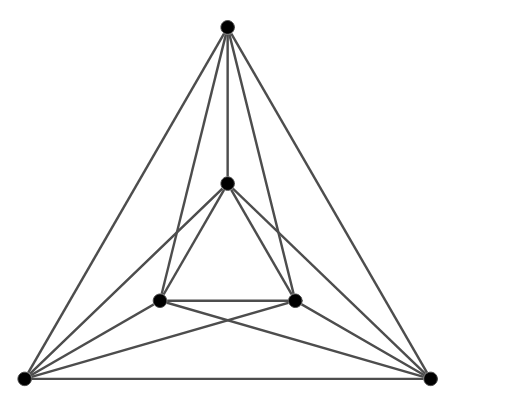
\includegraphics[width=5cm]{k6}\\
z rysunku wynika, że $\xi(K_6) \leq 3$ \\
Załóżmy zatem, że $\xi(K_6) = 2$, oba przecięcia dotyczą czterech różnych wierzchołków.  
Usuńmy zatem jeden z wierzchołków, wówczas otrzymujemy graf $K_5$ bez przecięć co jest sprzecznością.
Zatem $\xi(K_6)=3$

\subsection*{Graf planarny 5-regularny}
narysuj graf planarny 5-regularny \\\\ rozwiązanie: \\
jest to graf dwunastościan: \\
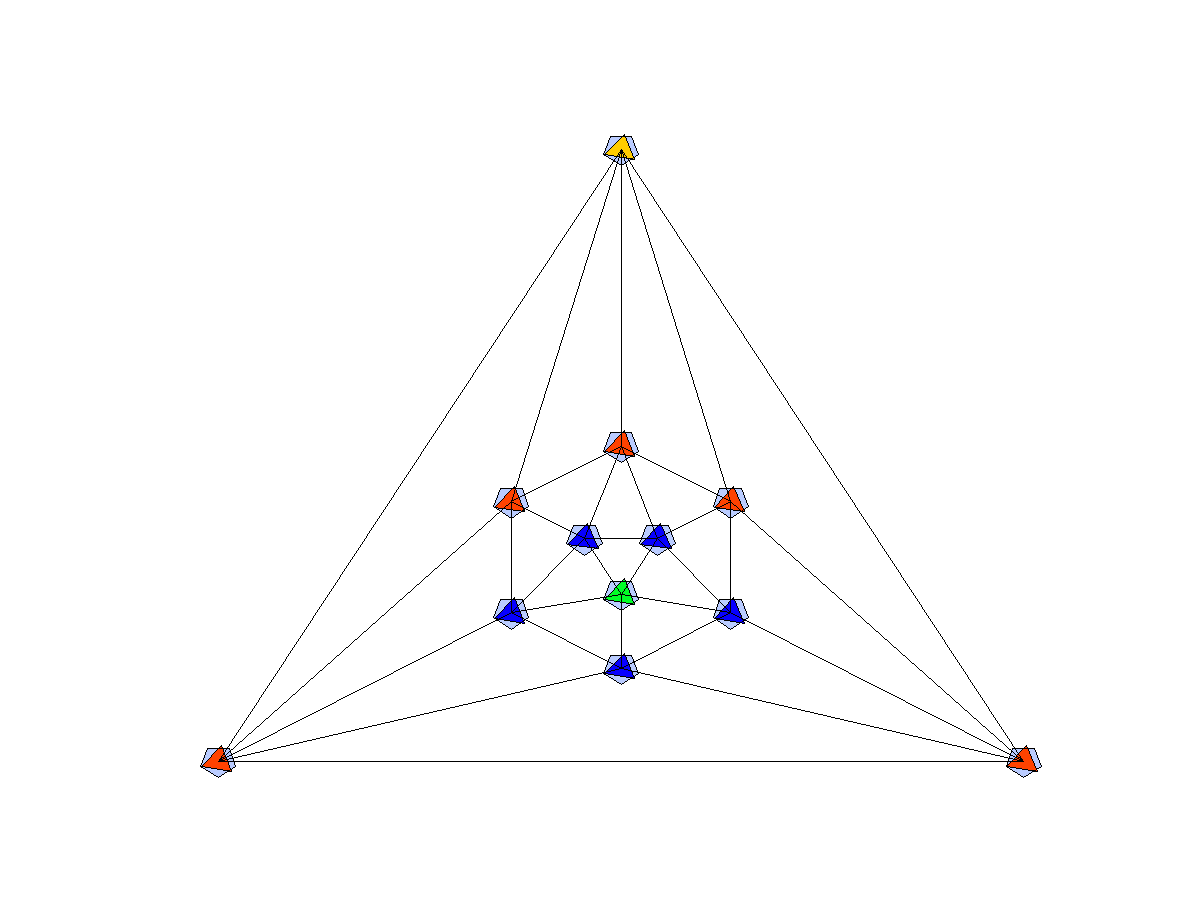
\includegraphics[width=5cm]{icosahedron} \\
warto zauważyć, że wszystkie grafy platońskie są planarne

\subsection*{Umieszczanie grafów}
Udowodnij, że graf może być umieszczony na płaszczyźnie $\iff$ może być umieszczony na powierzchni kuli. \\\\rozwiązanie:\\\\
($\longrightarrow$)\\
skoro graf może być umieszczony na płaszczyźnie to $\xi(G) = 0$ natomiast genus grafu ograniczony jest od góry $g \leq \xi(G) \rightarrow g = 0$ zatem można go również umieścić na kuli, która ma genus = 0\\\\
($\longleftarrow$) \\
skoro graf możemy umieścić na kuli, która jest powierzchnią bez rączek to znaczy, że nie ma przecięć więc można go również umieścić na płaszczyźnie \\\\
inne rozwiązanie:\\\\
każdą sferę można zrzutować na płaszczyznę z wyjątkiem jednego punktu (bieguna)



\subsection*{Znajdowanie klik w grafie kubicznym}
Zaprojektuj algorytm 1-absolutnie aproksymacyjny znajdujący największą klikę w n-wierzchołkowym grafie kubicznym. Algorytm powinien mieć złożoność $O(n)$ \\\\rozwiązanie:\\
Algorytm k-absolutnie aproksymacyjny -> algorytm taki, że dla danych I, gdzie OPT(I) - optymalny wynik, mamy $|A(I) - OPT(I)| \leq 1$, czyli musimy znaleźć algorytm, 
który będzie mógł się pomylić o 1 w zwracaniu rozmiaru kliki. Oto on:

\begin{lstlisting}
def clique(G):
	if n == 4:
		return {v1, v2, v3, v4}
	else:
		u = dowolnysasiad(v1)
		return {v1, u}
\end{lstlisting}
Czyli algorytm zwraca klikę $K_4$ lub $K_2$,  możliwe jest, że w grafie występuje $K_3$ ale chcemy stworzyć algorytm aproksymacyjny, więc możemy się pomylić o 1.
Algorytm ma złożoność $O(n)$, bo dowolnysasiad(v1) działa w czasie $O(n)$. Algorytm ma złożoność mniejszą niż złożoność pamięciowa, bo niewszystkie dane w macierzy 
sąsiedztwa reprezentującej graf są danymi istotnymi dla wyniku.

\subsection*{Nierówności trójkąta}
Dany jest zbiór n liczb. Sprawdź czy w tym zbiorze są takie 3, które mogą być długościami boków trójkąta. Algorytm powinien mieć złożoność $o(n^2)$. \\\\rozwiązanie:\\
\begin{lstlisting}
def triangle_inequality(A[1..n]):
	A = sort(A)
	c1 = A[1]
	c2 = A[2]
	for i = 3 to n:
		if c1 + c2 > A[i]
			return True
		else:
			c1 = A[i]
			swap(c1,c2)			
	return False

\end{lstlisting}
złożoność $O(nlogn)$

\subsection*{Najkrótszy cykl w grafie dwudzielnym}
Znajdź algorytm,  który w grafie $K_{p,q}$ ($p,q \ge 1$) znajdzie najkrótszy cykl i oszacuj jego złożoność obliczeniową.  
(rozważ przypadek a) lista sąsiedztwa, b) macierz sąsiedztwa)
Dlaczego jest ona mniejsza niż złożoność pamięciowa? \\\\rozwiązanie:\\
\begin{lstlisting}
def cykle(G):
	u1 = sasiad1(v)
	u2 = sasiad2(v)
	u3 = niesasiad(v)
	return (v, u1, u3, u2, v)
\end{lstlisting}
a)\\
złożoność obliczeniowa O(n) - przejrzenie sąsiedztwa v,  mniejsze niż n + m \\\\
b)\\
złożoność obliczeniowa O(n) mniejsze niż $n^2$ \\\\
złożoności obliczeniowe są mniejsze niż złożoność pamięciowa, bo zbiór danych nie składa się z samych danych istotnych

\subsection*{Harmoniczne kolorowanie}
Harmoniczne kolorowanie - to takie pokolorowanie grafu,  w którym:
\begin{itemize}
	\item sąsiednie wierzchołki mają różne kolory
	\item dowolne dwie krawędzie mają różne pary kolorów
\end{itemize}
Minimalną ilość kolorów do pokolorowania harmonicznie grafu oznaczamy $h(G)$ albo $\chi_H(G)$.  \\
Efektywną metodą na przechowywanie struktury grafu rzadkiego jest pokolorowanie go harmonicznie. 
Zapamiętujemy strukturę w postaci wektora kolorów W, gdzie $w_i \in W$ to kolor i-tego wierzchołka.
Obok wektora zapamiętujemy macierz C o rozmiarze $h(G) \times h(G)$, w której $c_{i,j} = (u,v)$ gdy uv
jest krawędzią o końcach pomalowanych kolorem i i kolorem j, w przeciwnym wypadku $c_{i,j} = 0$. 
Wiedząc, że $\sqrt{2m} < h(G) \leq n$ oszacuj:
\begin{enumerate}
	\item złożoność czasową procedury B(u,v) 
	\item złożoność pamięciową macierzy W i C
\end{enumerate}
rozwiązanie: \\\\
1)
\begin{lstlisting}
def B(v,u, W, C):
	kolor1 = W[v]
	kolor2 = W[v]
	if C[kolor1, kolor2] == 0:
		return false
	return true	
\end{lstlisting}
złożoność O(1) \\\\
2)\\
$M_W(n) = \theta(n)$ \\
$M_C(n) = \Omega(m) \cap O(n^2)$

\subsection*{Znajdowanie drogi długości k}
Posortuj złożoności malejąco dla algorytmu znajdowania drogi długości k w nieobciążonym grafie n-wierzchołkowym. \\
$O(4^k n^{O(1)})$, $O(k! n^{O(1)})$, $O(1,66^k n^{O(1)})$, $O((2e)^k n^{O(1)})$, $O(1,66^n n^{O(1)})$, $O(2^{3k/2} n^{O(1)})$, $O(2^k n^{O(1)})$ \\\\rozwiązanie:\\
ograniczenie górne na $k$: $k \leq n-1$ \\
$O(k! n^{O(1)})$, $O((2e)^k n^{O(1)})$, $O(4^k n^{O(1)})$, $O(2^{3k/2} n^{O(1)})$, $O(2^k n^{O(1)})$,  $O(1,66^n n^{O(1)})$, $O(1,66^k n^{O(1)})$


\subsection*{LGS}
Naszkicuj program lgs zwracający liczbę gwiazd spinających zawartych w G. Oszacuj jego złożoność w zależności od m i n 
dla macierzy sąsiedztwa, listy sąsiedztwa, pęków wyjściowych. \\\\rozwiązanie:\\

\begin{lstlisting}
def lgs(G):
	l = 0
	for v in G:
		if |N(v)| = n-1:
			l += 1
	return l
\end{lstlisting}
dla macierzy sąsiedztwa $O(n^2)$, dla listy sąsiedztwa $O(n + m)$, dla pęków $O(n)$

\subsection*{Cykl}
Napisz program, który stwierdza, czy graf G zapisany w macierzy sąsiedztwa wierzchołków jest cyklem i oszacuj jego złożoność obliczeniową. \\\\rozwiązanie:\\
\begin{lstlisting}
def is_cycle(G[1..n][1..n]):
	odwiedzone = tablica[1..n]
	licznik_odwiedzone = 0
	wyzeruj(odwiedzone)
	obecny_wierzcholek = 1
	while licznik_odwiedzone != n:
		odwiedzone[obecny_wierzcholek] = 1
		licznik_odwiedzone += 1
		licznik_odwiedzone = 
		licznik_sasiadow = 0
		do_odwiedzenia = -1
		for i = 1 to n:
			if B(obecny_wierzcholek, i):
				licznik_sasiadow += 1
				if not odwiedzone[i]:
					do_odwiedzenia = i

		if B(obecny_wierzcholek, 0) and licznik_odwiedzone = n:
			return true
		if do_odwiedzenia = -1:
			return false
		if licznik_sasiadow != 2:
			return false
	
	return false 
\end{lstlisting}

\section{$\alpha$-redukcja}
\subsection*{klika o rozmiarze $\leq$ k}
Mamy algorytm, który odpowiada na pytanie, czy graf G zawiera klikę $\leq$ k jeśli G ma gwiazdę spinającą.
Jak wykorzystać ten algorytm dla grafu, który nie ma gwiazdy spinającej? \\\\rozwiązanie:\\
Chcemy się dowiedzieć, czy graf ma klikę $\leq$ k. \\
Dokładamy do G gwiazdę spinającą, następnie pytamy o to, czy powstały graf ma klikę $\leq$ k-1.

\section{Dowody grafowe}

\subsection*{Tw. Eulera}
Udowodnij, że jeśli G jest spójnym grafem płaskim to $s = m - n + 2$\\\\ rozwiązanie: \\
indukcja względem m: \\
Jeśli m = 1, to n = 1 i mamy jedną ścianę (przypadek trywialny P(1)) \\
załóżmy P(m-1) \\
Rozważmy m-krawędziowy graf G.
Jeśli G jest drzewem to m = n - 1 oraz f = 1 (jest acykliczny) czyli mamy P(m).
Jeśli G zawiera cykl, usuńmy pewną krawędź należącą do cyklu,  G-e ma m-1 krawędzi i s-1 ścian.
Korzystamy z P(m-1) i mamy $s-1 = m-1 - n + 2 \rightarrow s = m - n + 2 \iff P(m)$. cnd

\subsection*{Lemat o pocałunkach}
Udowodnij, że dla każdego spójnego grafu płaskiego G o $n \geq 3$ zachodzi $2m \geq 3s$ \\\\rozwiązanie: \\
Dwa przypadki: \\
1)G jest drzewem (s=1)\\
zatem $m = n - 1 \leq 2 \rightarrow 2m \leq 4 = 4s \leq 3s$ \\
2) G zawiera cykl \\
usuwamy wszystkie wierzchołki stopnia 1 otrzymując w ten sposób $R(G)$ (rdzeń G). Każda jego ściana
jest otoczona przez co najmniej 3 krawędzie oraz s(R(G)) = s(G) czyli mamy $m(R(G))\geq 3s \rightarrow 2m(R(G)) \geq 3s$. 
Tym bardziej $m(G) \geq 3s$. cnd 

\subsection*{Przydatne ograniczenie górne na m}
Udowodnij, że dla grafu planarnego G o $n\geq 3$ mamy $m \leq 3n-6$ \\\\ rozwiązanie: \\
załózmy, że G jest płaski (jest izomorficzny do grafu płaskiego więc możemy tak zrobić) \\
mamy $s = m - n + 2$ oraz $2m \geq 3s$ \\
wstawiamy do lematu o pocałunkach wzór na s i otrzymujemy wzór z twierdzenia.  cnd

\subsection*{Własności drzewa}
Udowodnij, że następujące własności są równoważne: 
\begin{enumerate}
	\item T jest drzewem
	\item T jest acykliczny i ma n-1 krawędzi
	\item T jest grafem spójnym i ma n-1 krawędzi
	\item T jest grafem spójnym i każda krawędź jest mostem
	\item każde dwa wierzchołki T są połączone dokładnie jedną drogą
	\item dodanie do T jednej krawędzi stworzy dokładnie jeden cykl
\end{enumerate}
rozwiązanie:\\
wszystkie własności są trywialne dla n =1,  załóżmy prawdziwość wszystkich własności dla P(k), gdzie $k < n$ \\\\
($1. \rightarrow 2.$) \\
T jest z definicji acykliczne, po usunięciu dowolnej krawędzi otrzymujemy $T-e = T_1 \cup T_2$ (rozspajamy). 
Z założenia indukcyjnego $m(T-e) = m(T_1) + m(T_2) = n(T_1) + n(T_2) - 2 \rightarrow m(T) = n(T_1)+n(T_2)-1 = n(T) - 1$ zatem 
$m = n-1$ \\\\
($2. \rightarrow 3.$) \\
 zakładamy,  że T nie jest grafem spójnym zatem $T = T_1 \cup T_2$
z założenia indukcyjnego $m(T) = m(T_1) + m(T_2) = n(T_1) + n(T_2) - 2 \rightarrow m = n-2$ co jest sprzeczne z 2. 
zatem T musi być spójny. \\\\
($3. \rightarrow 4.$) \\
k = 1 - ilość składowych spójności, czyli minimalna ilość krawędzi, która czyni go spójnym to n-1 więc każda krawędź musi być mostem\\\\
($4. \rightarrow 5.$) \\
załóżmy, że między pewną parą wierzchołków mamy dwie drogi, zatem jeśli usuniemy którąś z krawędzi należących do jednej z dróg to 
nie rozspoimy grafu co jest sprzeczne z 4. \\\\
($5. \rightarrow 6.$) \\
załóżmy, że T zawiera cykl, wtedy dwa wierzchołki należące do tego cyklu połączone są dwiema różnymi drogami co jest sprzeczne
z 5.  po dodaniu krawędzi między tymi wierzchołkami tworzymy cykl,  bo mamy jedną drogę, która była wcześniej i nową drogę przez tą 
krawędź,  zatem $\gamma = 1$ \\\\
($6. \rightarrow 1.$) \\
załóżmy, że graf nie jest spójny, jest to sprzeczne z 5. bo dodanie jednej krawędzi nie gwarantuje stworzenia cyklu, 
zatem T musi być spójny, z 6. jest również acykliczny zatem jest drzewem \\\\

\subsection*{Pąki w grafie planarnym}
Udowodnij, że każdy graf planarny zawiera co najmniej 3 pąki (pąk - wierzchołek v taki, że $deg(v) \leq 5$ \\\\
rozwiązanie:\\
załóżmy, że mamy w grafie planarnym tylko dwa pąki v i u,  zatem 
$deg(v) + deg(u) + 6(n-2) \leq 2m \leq 6n - 12 $ co jest sprzeczne ($deg(v) \ne 0$ i $deg(u) \ne 0)$ (ostatnia nierówność z przydatnego oszacowania górnego m) 

\subsection*{Liczba cyklomatyczna}
Udowodnij, że dla dowolnego grafu spójnego liczba cyklomatyczna $\gamma(G) = m - n + 1$ \\\\ rozwiązanie: \\
usuwamy tyle krawędzi, żeby graf stał się acykliczny (czyli żeby stał się drzewem), w drzewie m = n - 1, czyli musimy usunąć m - (n-1) krawędzi cnd. 

\section{Trudne zadania}
\subsection*{Pokrycie wierzchołkowe *}
Algorytm rozwiązuje problem k-pokrycia wierzchołkowego grafu G
\begin{lstlisting}
def vertexcover(G,k)
	if E(G) empty: 
		return true
	if k == 0:
		return false
	wybierz dowolne e = uv
	return vertexcover(G - u,  k - 1) or vertexcover(G - v, k - 1)
\end{lstlisting}
\begin{enumerate}
	\item jaka jest złożoność algorytmu w terminach m i k
	\item podaj typy grafów i wartości k, dla których vertexcover zwraca true w czasie wielomianowym
	\item podaj typy grafów i wartości k, dla których vertexcover zwraca false w czasie wykładniczym
\end{enumerate}

\subsection*{MFP}
W historii problemu maksymalnego przepływu znane są m.in.  następujące algorytmy:\\
(1969) Edmondsa-Karpa \\
(1970) Dinica \\
(1974) Karzanova \\
(1977) Cherkaskyego \\
(1978) Galila \\
(1978) Shiloacha \\
(1980) Sleatora-Tarjana \\
(1986) Goldberga-Tarjana \\
(2013) Orlina \\
o złożonościach $O(nm)$, $O(nmlog(n^2/m)),$ $O(nmlogn)$, $O(nmlog^2n)$, $O(n^{5/3}m^{2/3})$, $O(n^2\sqrt m)$, $O(n^3)$, $O(n^2m)$, $O(nm^2)$ \\
przyporządkuj złożoności do odpowiednich algorytmów \\\\ rozwiązanie: \\
trzeba rozpatrzeć dwa przypadki: 1. grafy rzadkie, 2. grafy gęste i średnio gęste

\subsection*{Listowa reprezentacja drzew n-wierzchołkowych}
Zaproponuj listowy sposób reprezentacji drzew n-wierzchołkowych w pamięci O(n) umożliwiający sprawdzanie O(1), 
czy para wierzchołków jest połączona krawędzią. 

\subsection*{Minimalne rozcięcie}
Problem Minimalne Rozcięcie pyta jak równo podzielić wierzchołki grafu, tak aby zminimalizować liczbę krawędzi łączących wierzchołki z różnych podzbiorów.
Najszybszy znany algorytm dla problemu MR ma złożoność $O(2^{O(kkk}n^3log^3n)$ gdzie k jest rozmiarem minimalnego cięcia. Jaka jest najszersza klasa grafów, 
dla której problem MR jest wielomianowy? Jaki jest wówczas zwiącek pomiędzy k i n? Jaka jest wówczas złożoność wspomnianego algorytmu? \\\\rozwiązanie:\\
jakie to mogą być klasy? \\
$K_{p,q}$: k = 0, T = $O(n^3log^3n)$ \\
$T_n$: k = 1,  T = $O(n^3log^3n)$ \\
$Q_p$: $k = logn$, T = $O(n^6log^3n)$ \\
$N_n$: $k = 0$


\end{document}
